\section{User Interface}
The user interface (UI), as shown in \Cref{fig:figure1}, is where the analysis
is configured and managed. Here, the user is able to provide the necessary
parameters to create the simulation, start the simulation both locally and
remotely, and view the simulation results. The interface contains several
separate areas:

\begin{figure}[!htbp]
  \centering {
    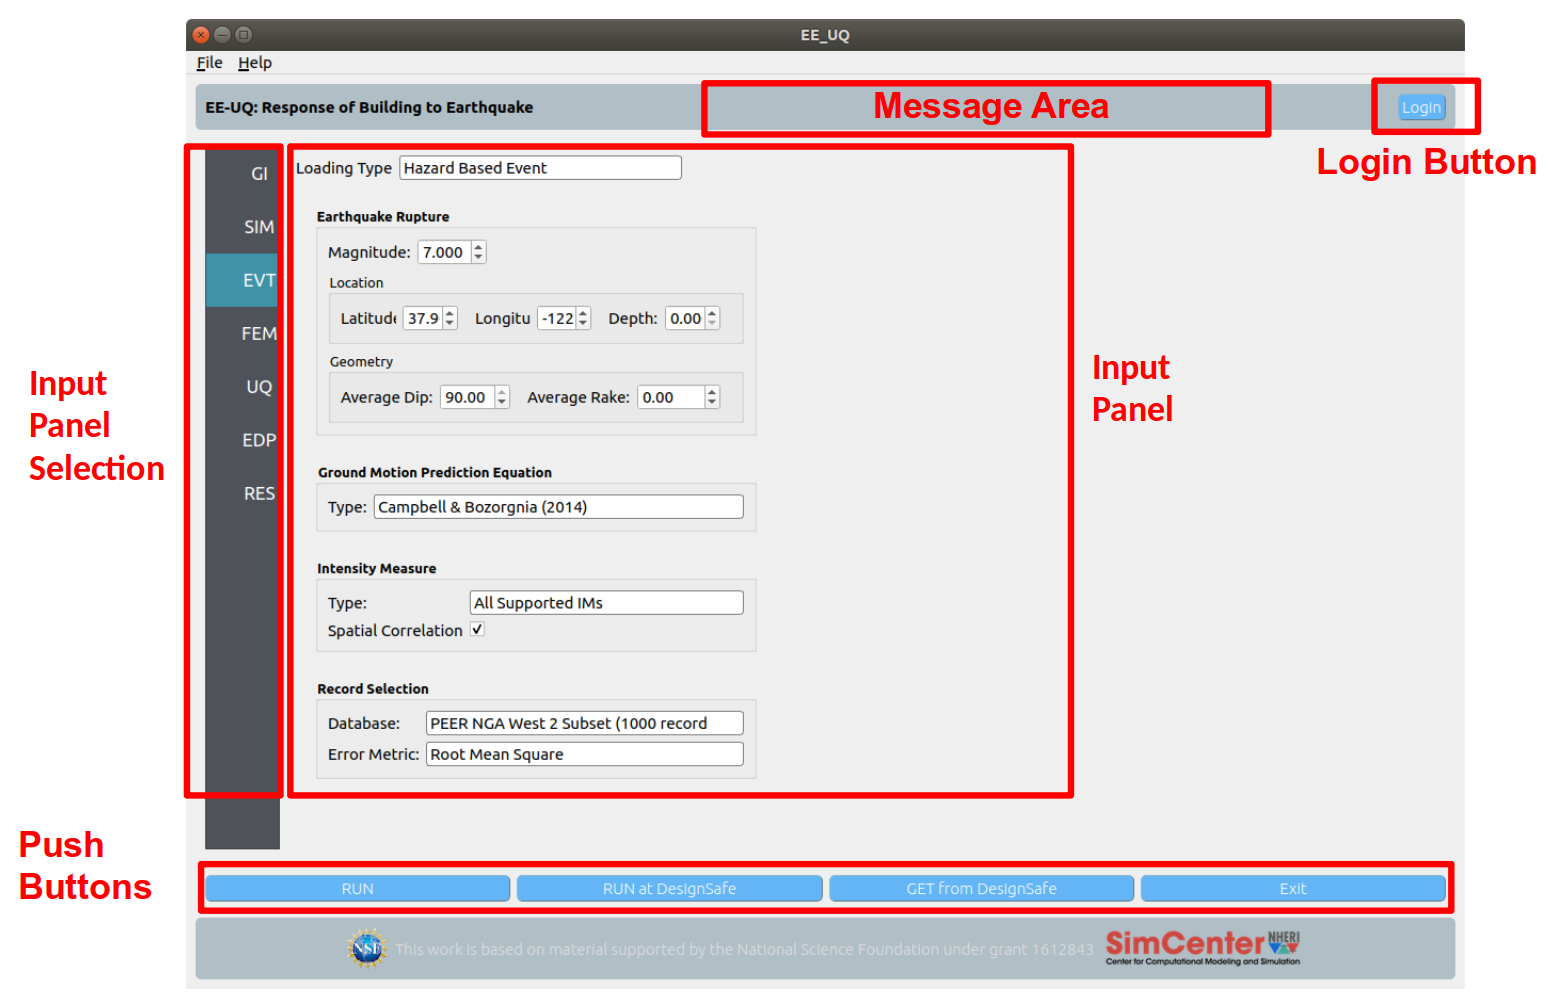
\includegraphics[width=0.8\textwidth]
    {usage/figures/ui.png} }
  \caption{UI}
  \label{fig:figure1}
\end{figure}

\begin{enumerate}
\item Input Panel Selection: This area on the left side provides the
  user with a selection of items to choose from from:
\begin{enumerate}
  \item GI: General Information (\ref{sec:generalInfo}), for specifiction of building
    description, location and units.
  \item SIM: Structure Information Model (\ref{sec:structuralInfo}), for description of the
    building model.
  \item EVT: Event (\ref{sec:event}), for selecting the input earthquake motions for building.
  \item FEM: Finite element method (\ref{sec:fem}), for specifying the analysis options.
  \item UQ: Uncertainty quantification (\ref{sec:uq}), for defining the distribution
    of the random variable paramaters and UQ method analysis options.
  \item EDP: Engineering Demand Parameters (\ref{sec:edp}), for specification of
    output response quantities.
  \item RES: Results output (\ref{sec:results}), for looking at the results.
\end{enumerate}

Selecting any of these will change the input panel presented.

\item Input Panel: This is the large central area of the UI that the
  user provides input for the application chosen and views the
  results. For example if the user had selected UQ in the input panel
  selection, it is in this panel that the user would provide details
  on the distributions associated with each random variable or select
  the sampling method to use and provide the options necessary to run
  that method.

\item Push Buttons: This is the area near the bottom of the UI in
  which 4 buttons are presented to the user:

\begin{enumerate}
\item RUN – to run the simulation of the user’s desktop machine.
\item RUN at DesignSafe – to process the information, and send to
  DesignSafe where the job will be run on a supercomputer and results
  stored in your DesignSafe jobs folder.
\item GET from DesignSafe – to obtain from DesignSafe your list of
  jobs and select from that list a job to download.
\item Exit: to exit the application.
\end{enumerate}

The use of the push buttons is discussed in \Cref{sec:push_buttons}.

\item Login Button: At the top right of the UI is the login
  button. Before the user can launch any jobs on DesignSafe, they must
  first login to DesignSafe using their DesignSafe login and
  password. Pressing the login button will open up the login window
  for users to enter this information. Users can register for an
  account on
  the \href{https://www.designsafe-ci.org/account/register/}{DesignSafe
  webpage}.

\item Message Area: In the top center of the application is the area
  of the interface that error and status messaged will be displayed
  while the application is running.

\end{enumerate}


\section{GI: General Information}
The user here provides information about the building and the units
the user will work in. The widget itself presents 3 separate frames,
as shown in \autoref{fig:figure2}, to the user:

\begin{enumerate}
\item Building Information frame in which user provide general information about the building, this include year of construction and type.
\item Properties frame in which user provides information about number of stories, width, depth, plan area and height of the building.
\item Location frame in which user provides location of the building. This information is used in some of event widgets to obtain events specific to the building.
\item Units frame  in which user specifies what the units will be for the inputs and outputs. Some widgets will require inputs in different units. These entries will contain units beside the specific entry to mark this.
\end{enumerate}


\begin{figure}[!htbp]
  \centering {
    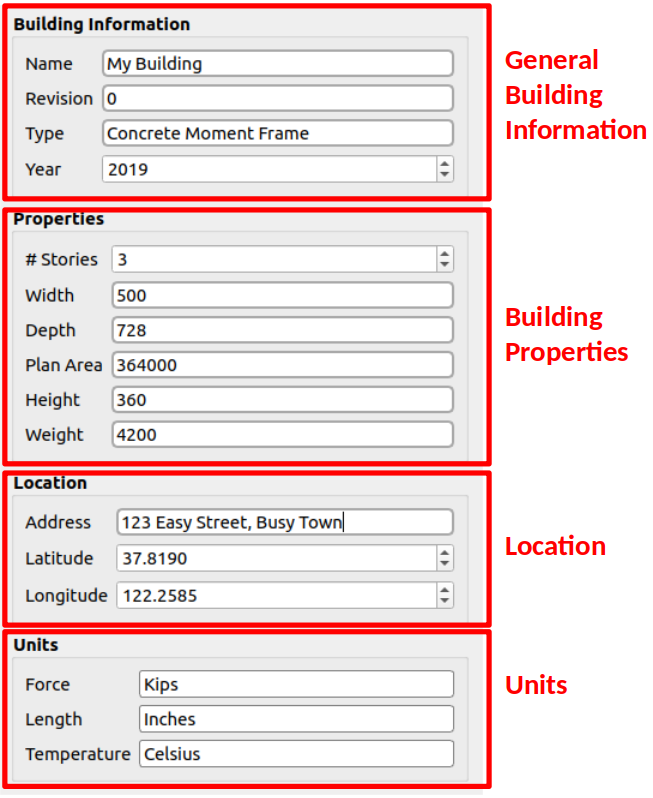
\includegraphics[width=0.5\textwidth]
    {usage/figures/gi.png} }
  \caption{BIM}
  \label{fig:figure2}
\end{figure}



\section{SIM: Structural Information Model}
This panel is where the user defines the structural model of the
building. The structural model is that part of the building provided
to resist the lateral loads. There are a number of backend
applications provided for this part of the workflow, each responsible
for providing the structural analysis model to the workflow. The
drop-down menu at the top of this panel is where the user selects
which application to use. As the user switches between applications,
the entry data changes to reflect the different inputs the different
applications require. At present there are two backend applications
available through the drop down menu: 

\begin{enumerate}
\item Multiple Degrees of Freedom (MDOF) (\ref{sec:MDOF})
\item \texttt{OpenSees} (\ref{sec:OpenSeesSIM})
\end{enumerate}

\subsection{Multiple Degrees of Freedom (MDOF)}\label{sec:MDOF}

This panel is provided for users to quickly create simple shear models
of a building. The panel, as shown in \Cref{fig:mdof} is divided
into 3 frames:
\begin{enumerate}
\item In the top left frame the user enters the number of stories. For
  each story the user then enter the story height, initial stiffness in
  1 and 2 directions, yield strength in the 1 and 2 directions, and
  hardening ratio again in the 1 and 2 directions. Here, the 1 and 2 directions
  are the orthogonal $x$ and $y$ axes in plan view. In addition, user enters
  the floor weights and damping ratios for each of the nodes.
\item In the lower left frame the user has the option of overriding an
  individual floor or story basis, or any of the properties set in the
  upper frame.
\item On the right side of the frame is a graphical widget showing the
  current building. When entering data into the lower left frame,
  those floors and stories corresponding to data being modified is
  highlighted in red.
\end{enumerate}

\begin{figure}[!htbp]
  \centering {
    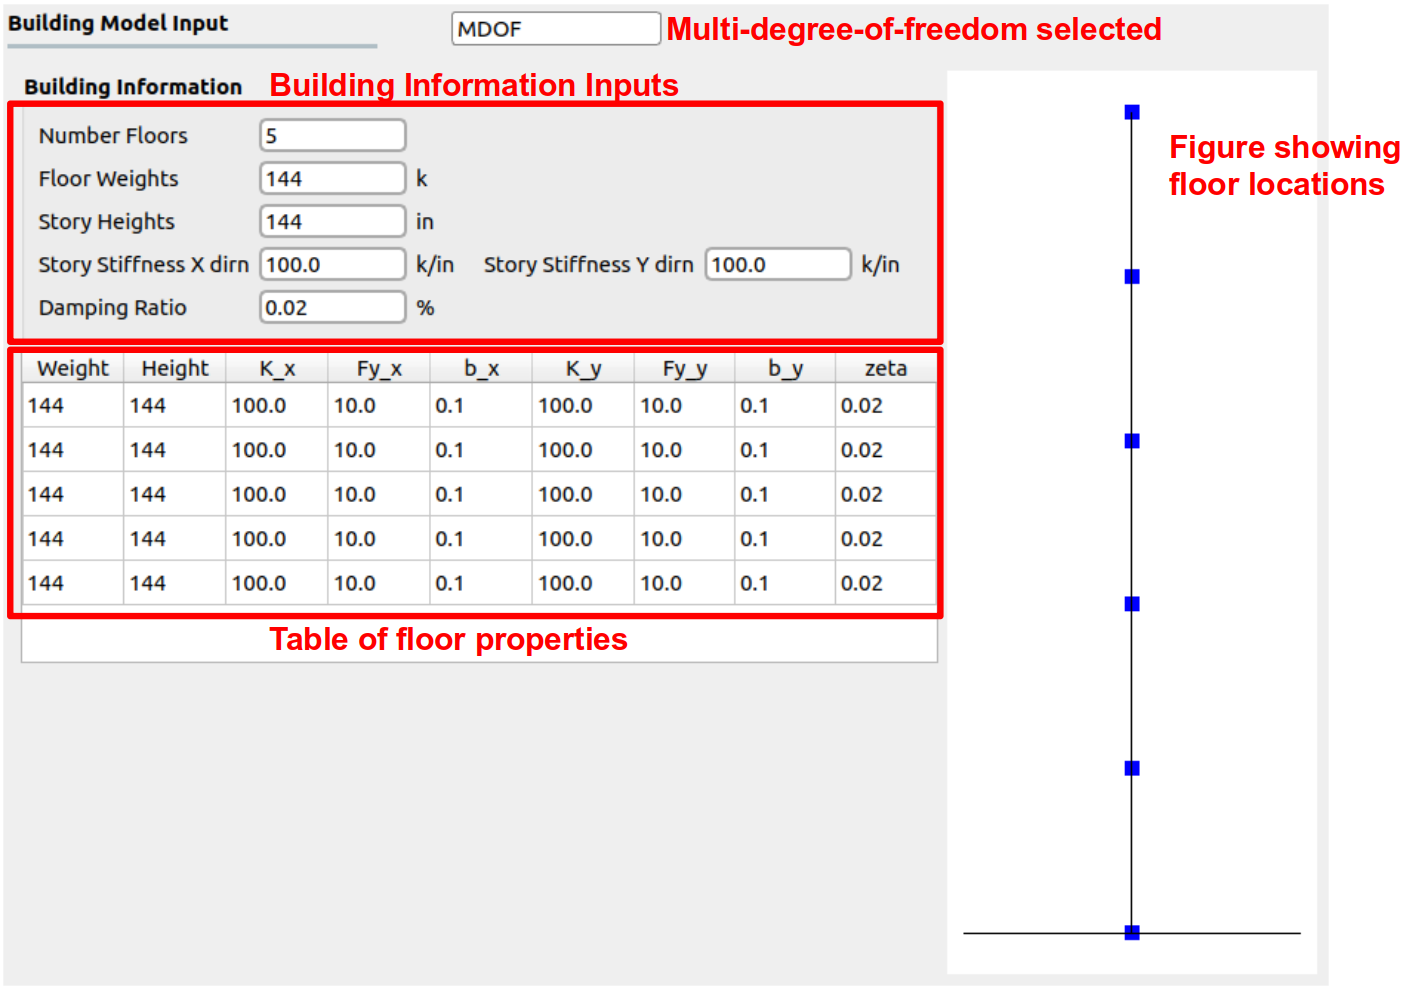
\includegraphics[width=0.8\textwidth]
    {usage/figures/mdof.png} }
  \caption{MDOF or Shear Building Model}
  \label{fig:mdof}
\end{figure}

Random Variables: Random Variables can be created by the user entering
a valid string instead of a number in the entry fields for all entries
except the number of floors. The variable name entered will appear as
a Random Variable in the UQ panel and it is there that the user must
enter the distribution for the Random Variable.

\subsection{\texttt{OpenSees}}\label{sec:OpenSeesSIM}
This panel is for users who have an existing \texttt{OpenSees} model of a
building that performs a gravity analysis and now wish to subject that
building model to one of the \texttt{EVT} options provided. The input panel
for this option is shown in \Cref{fig:figure3}. The user has 3 fields
that they need to complete:
\begin{enumerate} 
\item The user specifies the main script that contains the building
  model. This script should build a model and perform any gravity
  analysis of the building that is required before the event is
  applied.
\item A list of nodes that define a column line of interest for which
  the responses will be determined. The column nodes should be in
  order from ground floor through to roof. The EDP options, described
  in \Cref{sec:edp}, use this information to determine nodes at which
  displacement, acceleration and story drifts are calculated.
\item An entry for the dimension of the model, i.e. 1D, 2D or 3D. This
  information is used to apply ground motions.
\end{enumerate}

\begin{figure}[!htbp]
  \centering {
    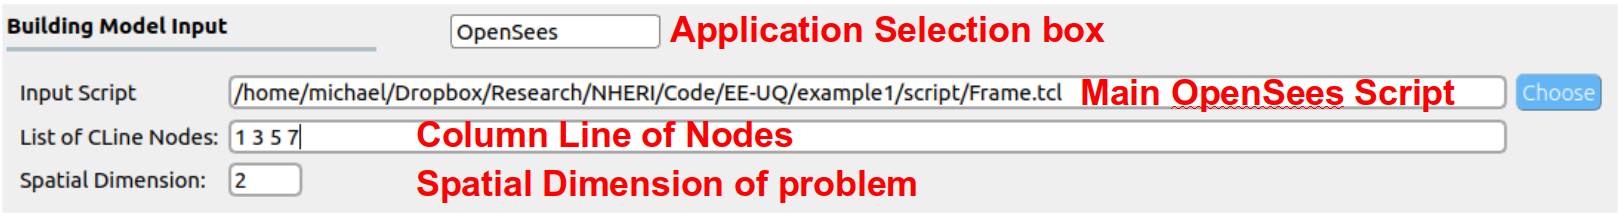
\includegraphics[width=0.8\textwidth]
    {usage/figures/openSees.png} }
  \caption{\texttt{OpenSees} Model}
  \label{fig:figure3}
\end{figure}

Random Variables: In \texttt{OpenSees} there is an option to set
variables to have certain values using the \texttt{pset} command, e.g
\texttt{pset a 5.0} will set the variable a to have a value 5 in an
\texttt{OpenSees} script. In \texttt{\getsoftwarename{}}, any variable
found in the main script to be set using the \texttt{pset} command
will be assumed to be a Random Variable. As such, when a new main
script is loaded all variables set with \texttt{pset} will appear as
Random Variables in the UQ panel.


\section{EVT: Event}
The event panel presents the user with a drop-down menu with a list of
available event applications. Event applications are applications
that, given the building and user supplied data to the specific
applications input panel, will generate a list of events for the
building. There are a number of options available in the pull-down
menu.

\subsection{Multiple Existing}
This panel is provided for the user to specify multiple existing SimCenter
event files.  If more than one event is specified it is done to
provide the UQ engine with a discrete set of events to choose
from\textemdash it is not done with the intention of specifying that
one event follows another.  The panel presented to the user
is shown in \Cref{fig:SC_event_panel}.

\begin{figure}[!htbp]
  \centering {
    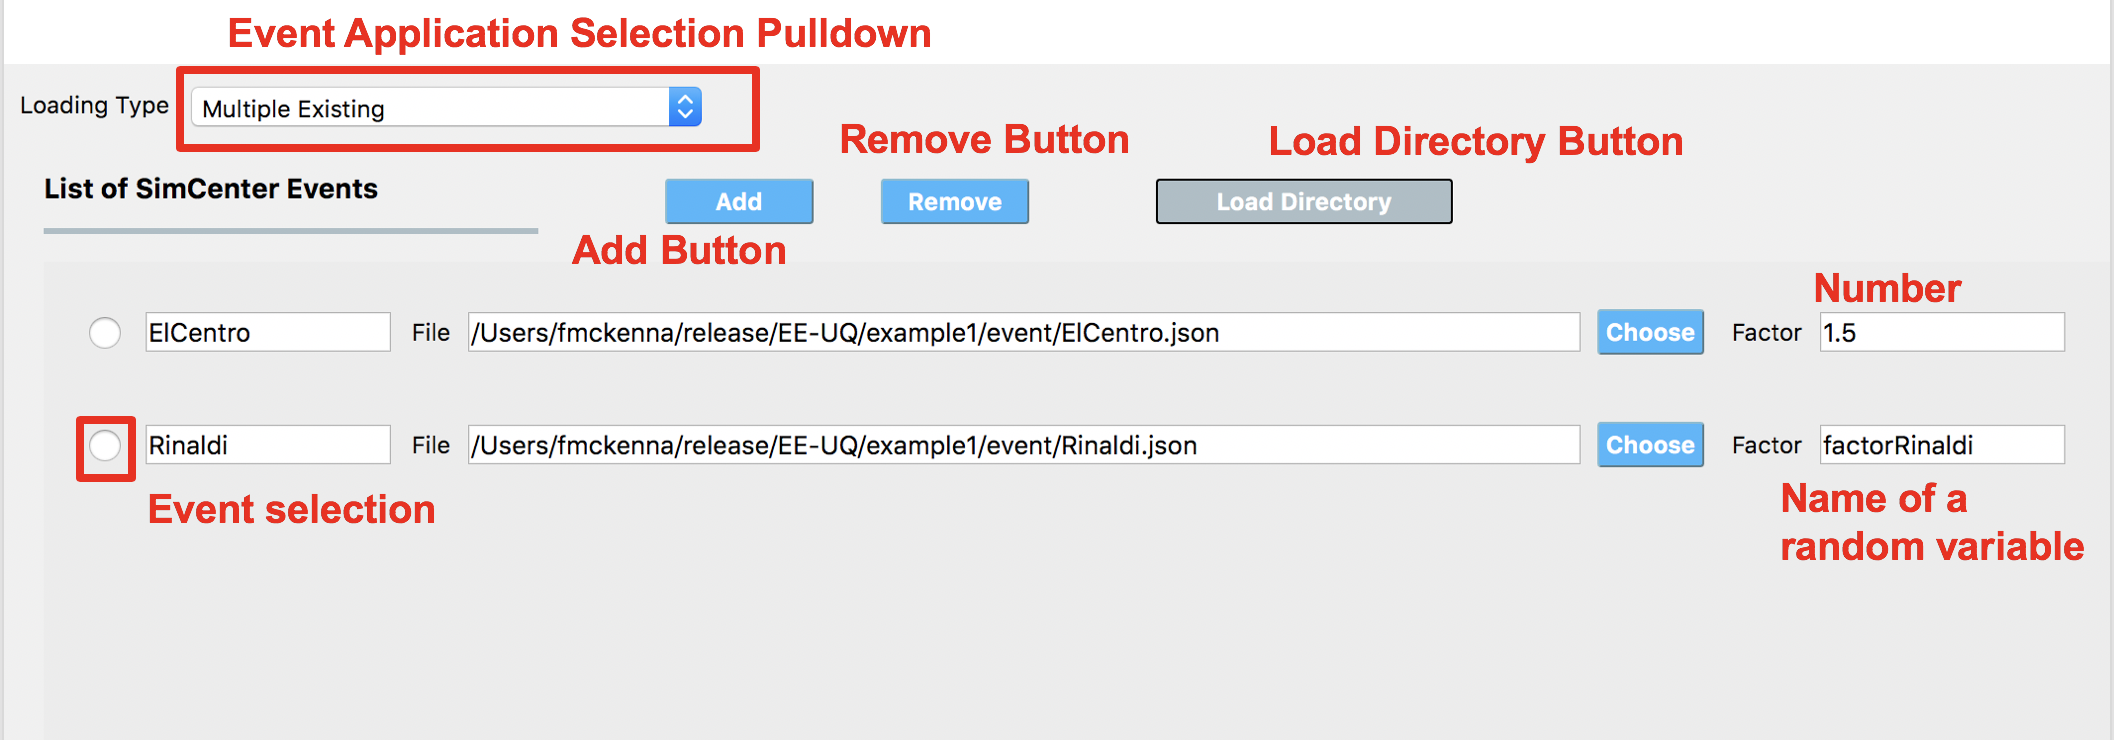
\includegraphics[width=0.8\textwidth]
    {usage/figures/multipleExisting.png} }
  \caption{Multiple Existing (SimCenter) Events }
  \label{fig:SC_event_panel}
\end{figure}

Use the \texttt{Add} button to add a new event. This adds an empty
event to the panel. Pressing the button multiple times will keep
adding events to the panel. \Cref{fig:SC_event_panel} shows the state after
the button has been pressed twice, and data entered to load the El Centro
and Rinaldi Events.

The path to the event file can be entered manually, or using the \texttt{Choose} button for convenience. Pushing the button brings up a typical file search screen. By default, a scale factor of 1.0 is assigned to the event.  The user
can change this to another floating point value (DO NOT USE INTEGER), and they can define the scale factor as a random variable by
entering a variable name, such as \texttt{factorRinaldi} for the second event in \Cref{fig:SC_event_panel}.

Note: the name of the random variable must not start with a number, or contain any spaces or special characters, such as -, +, \%, etc.

The \texttt{Remove} button is used to remove events. To remove an
event, the user must first select events they wish to remove,
which is done by clicking in the small circle at the left side of the event frame. All of the selected events are removed when the \texttt{Remove} button is pressed.

The \texttt{Load Directory} button provides a convenient method to load multiple events. All event files shall first
be placed into the same folder. We recommend to put the files in a folder of their own, with no other files besides the earthquake events in it. After pressing the \texttt{Load Directory} button, the user will be able to choose the directory that contains the files, and the
application will load all event files (i.e., every file with a \texttt{.json} 
extension) into the widget automatically. 

Initially, every
event will be given a load factor of 1.0. Load factors can be assigned automatically by preparing a \texttt{Records.txt} file in the directory with the events. Each line in the \texttt{Records.txt} shall represent one event file, and contain two comma separated values: the event file name and the desired scale factor. The application will open that file automatically and assign the prescribed load factors to the events. Using a \texttt{Records.txt} file also allows users to load only a subset of the events from a folder by listing only those in the file. An example \texttt{Records.txt} is shown below:

\begin{verbatim}
ElCentro.json,1.5
Rinaldi.json,2.0
\end{verbatim}

Random Variables: Scale factors can be defined as being random variables by entering a string in the factor field. The variable name entered will appear as a Random Variable in the UQ panel and the user must specify its distribution there. If multiple
events are specified, the event itself will be also be treated as a random
variable, with each event being part of the discrete set of possible
events. For discrete events the user does not define a distribution, this is done automatically.


\subsection{Multiple PEER Event}
This event option is provided for the user to specify multiple existing
\href{http://peer.berkeley.edu}{PEER} ground
motion files.  For PEER events, the user is required to specify the
individual components for the EVENTS.  The \texttt{Add/Remove} buttons
at the top are to create and remove an event, as
per \Cref{subsec:multiple_existing}. For the PEER events, the user
specifies components acting in the individual degree-of-freedom
directions.  The \texttt{+} and \texttt{-} buttons add and remove
components with remove removing all components selected. Each
component in a PEER event can have their own scale factor, again a
number or a random variable.

\begin{figure}[!htbp]
  \centering {
    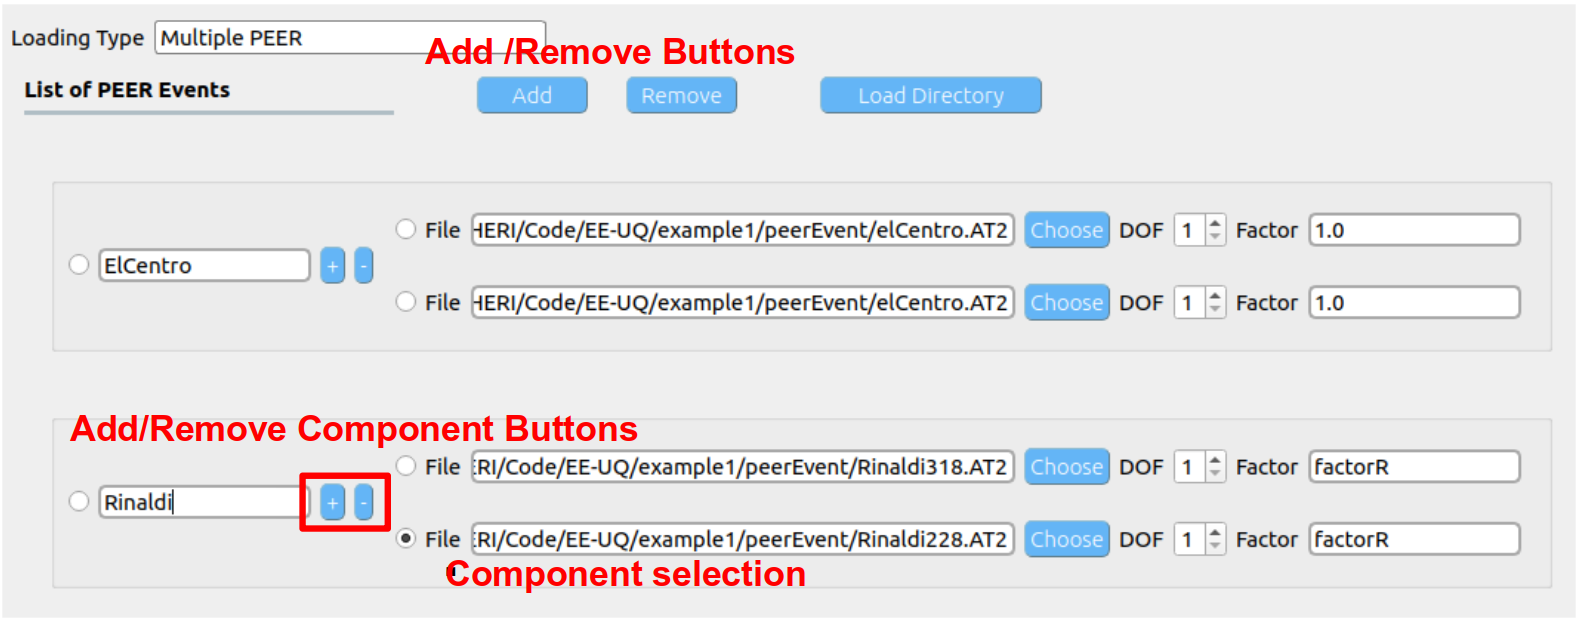
\includegraphics[width=0.8\textwidth]
    {usage/figures/multiplePEER.png} }
  \caption{\texttt{Multiple PEER} loading type}
  \label{fig:figure6}
\end{figure}

If the user has multiple events to load, they can again place all the
PEER \texttt{.AT2} files into a separate folder and select
the \texttt{Load Directory} option. This will allow the user to select
a directory. Once selected, all \texttt{.AT2} files in that directory will be
loaded into the application. Similar to loading multiple SimCenter
events, should the user provide a file \texttt{Records.txt} in that
directory, the application will load all files in the list and set the
appropriate load factor. An example \texttt{Results.txt} file for multiple Peer
events is as shown below:

\begin{verbatim}
elCentro.AT2,1.5
Rinaldi228.AT2,2.0
Rinaldi318.AT2,2.0
\end{verbatim}

Random Variables: The user can, as mentioned, enter a string in the
factor field to specify that the factor is to be considered a random
variable. Subsequently, in the UQ panel the user must provide
information on the random variables distribution. Also, if multiple
events are specified, the event itself will be treated as a random
variable with each event being part of the discrete set of possible
events.


\subsection{Hazard Based Event}
The panel for this event application is as shown in
\autoref{fig:figure7}.  This application implements a scenario-based
(deterministic) seismic event.  In this panel the user specifies an
earthquake rupture (location, geometry and magnitude), a ground motion
prediction equation, a record selection database and the intensity
measure used for record selection.  In the backend, this application
relies on three other applications to perform seismic hazard analysis,
intensity measures simulation (to create a simulated target spectrum),
and ground motion record selection/scaling.  Users interested in
learning about those applications are referred to the documentation of
the
(\href{https://github.com/NHERI-SimCenter/GroundMotionUtilities/blob/master/Readme.md}{SimCenter
  ground motion utilities}).

\begin{figure}[!htbp]
  \centering {
    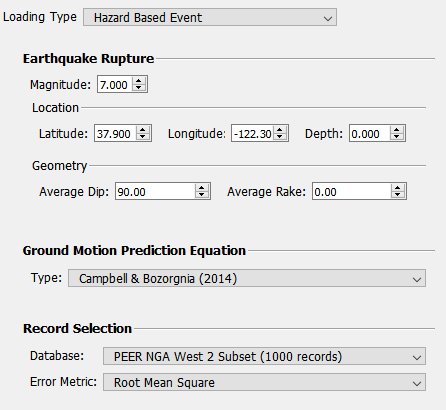
\includegraphics[width=0.8\textwidth]
    {usage/figures/hazardBased.png} }
  \caption{\texttt{Hazard Based Event} loading type}
  \label{fig:figure7}
\end{figure}


\subsection{Stochastic Ground Motion Model}
This option allows users to generate synthetic ground motions for a
target seismic event. In order to do so, the stochastic ground motion
model is selected from the drop-down menu, as shown
in \Cref{fig:stochastic_loading}. Depending on the model selected, the
user will be asked to enter values for a number of parameters that are
used to generate a seismic event. In the current release, users can
select between the model derived by Vlachos et
al. (2018) \cite{vlachos2018predictive} and the model developed by
Dabaghi \& Der Kiureghian (2014, 2017, 2018)
[\cite{dabaghi2014stochastic}, \cite{dabaghi2017stochastic}, \cite{dabaghi2018simulation}]. Additionally,
users can provide a seed for the stochastic motion generation if they
desire the same suite of synthetic motions to be generated on multiple
occasions.  If the seed is not specified, a different realization of
the time history will be generated for each run. The backend
application that generates the stochastic ground motions relies
on \texttt{smelt}, a modular and extensible C++ library for generating
stochastic time histories. Users interested in learning more about the
implementation and design of
\texttt{smelt} are referred to its
\href{https://github.com/NHERI-SimCenter/smelt}{GitHub repository}.

All input parameters can be specified as random variables by entering
a string in the parameter field. Please note that information for the
inputs that are identified as random variables needs to be provided in
the \texttt{UQ} tab.

\begin{figure}[!htbp]
  \centering {
    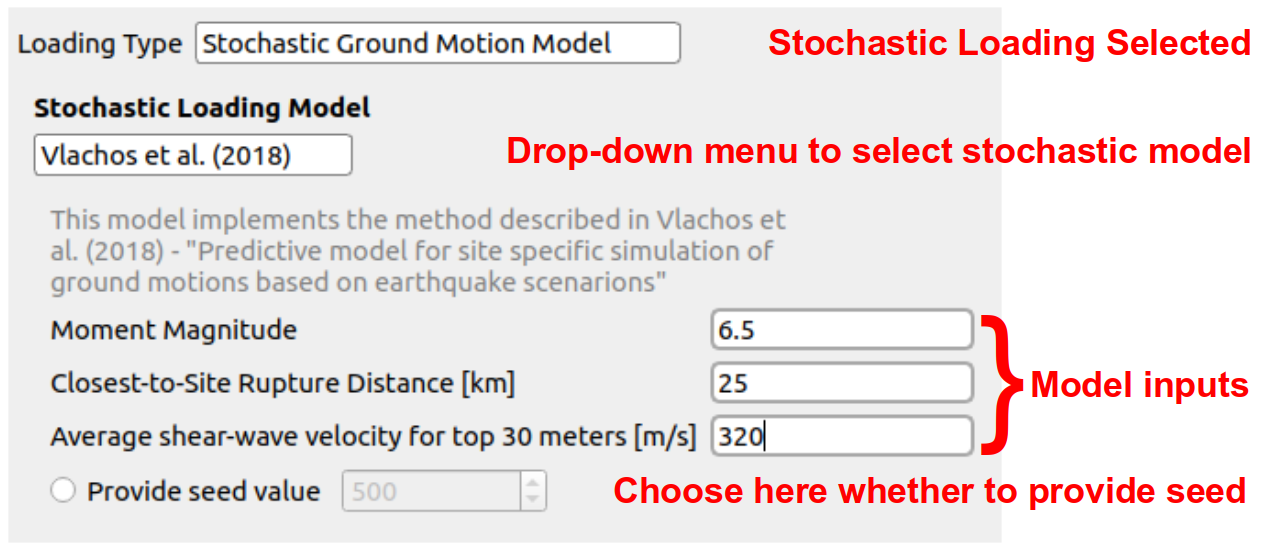
\includegraphics[width=0.8\textwidth]
    {usage/figures/stochastic_loading.png} }
  \caption{Stochastic Ground Motion Event}
  \label{fig:stochastic_loading}
\end{figure}


\subsection{Site Response}
The panel for this event application is as shown in \Cref{fig:s3hark0}. 
This application does effective free-field site response analysis of a soil column.
In this panel the user specifies a ground motion at the bottom of the column. 
With soil layer properly defined, the motion at the ground surface will be given at the end of the analysis.
\begin{figure}[!htbp]
  \centering {
    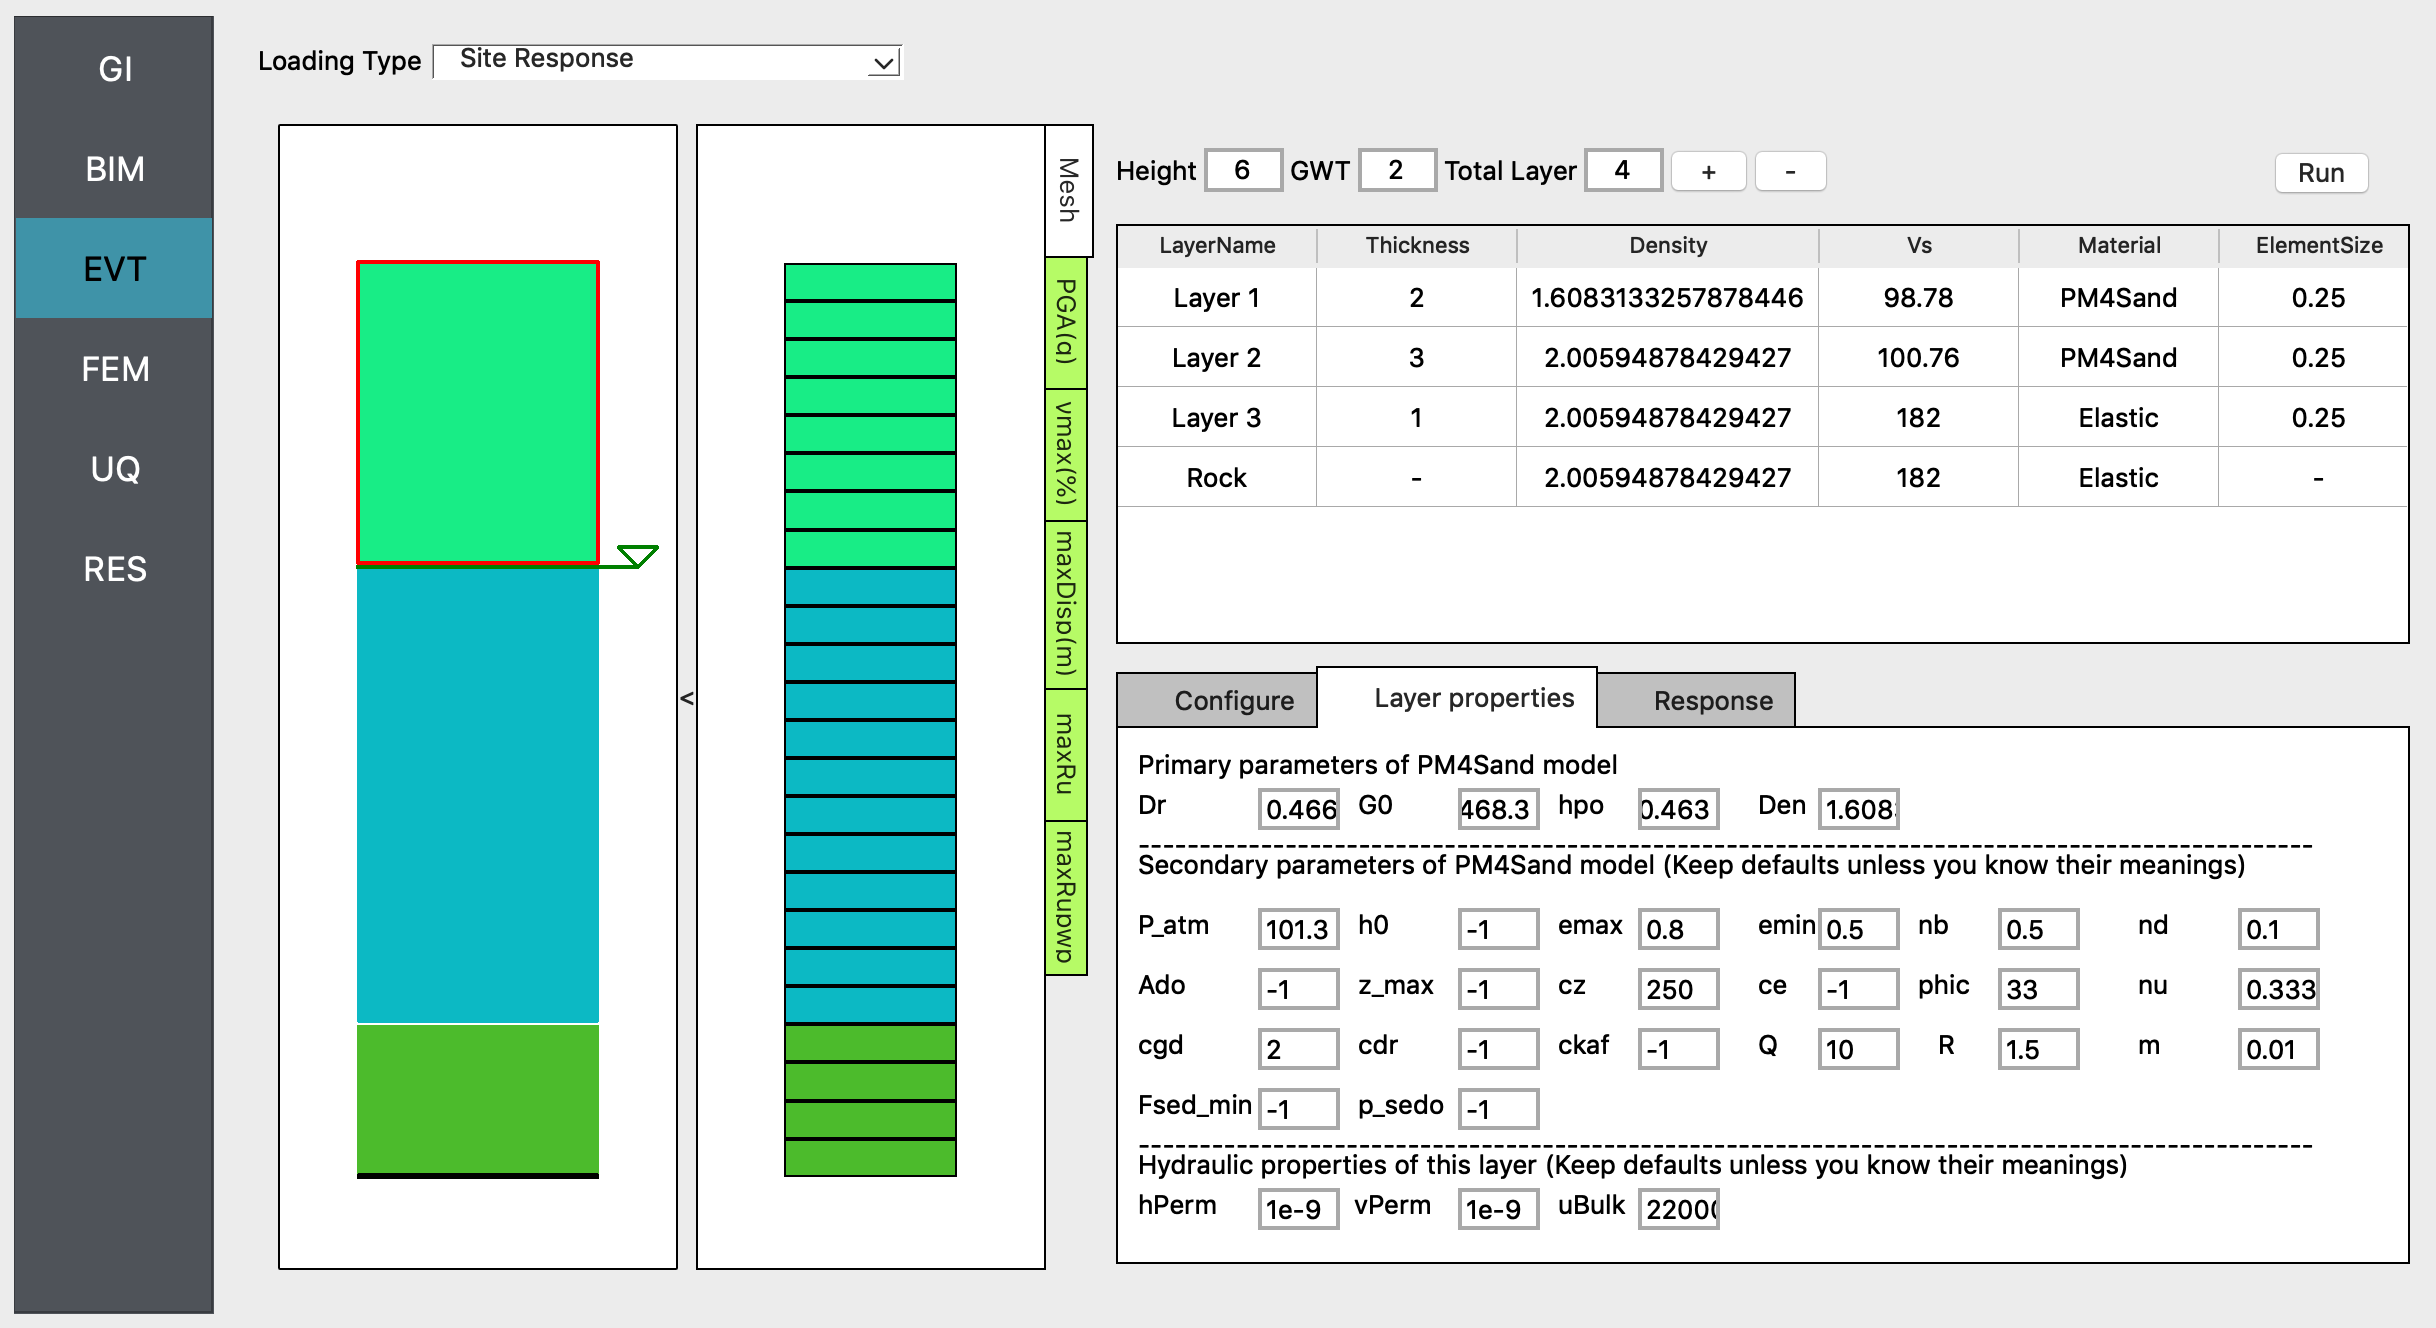
\includegraphics[width=0.8\textwidth]
    {usage/figures/s3hark0.png} }
  \caption{s$^3$hark}
  \label{fig:s3hark0}
\end{figure}

The UI of s$^3$hark is shown in \Cref{fig:s3hark1}.
There are two graphics shown in the left of the panel. The first one is the soil column graphic, 
which shows a visualization of the soil column.
The second one is the mesh and profile graphic, 
which shows the finite element mesh and profile plots.
On the right of the panel are operation area, soil design table, configure tab, layer property tab and response tab. 


\begin{figure}[!htbp]
  \centering {
    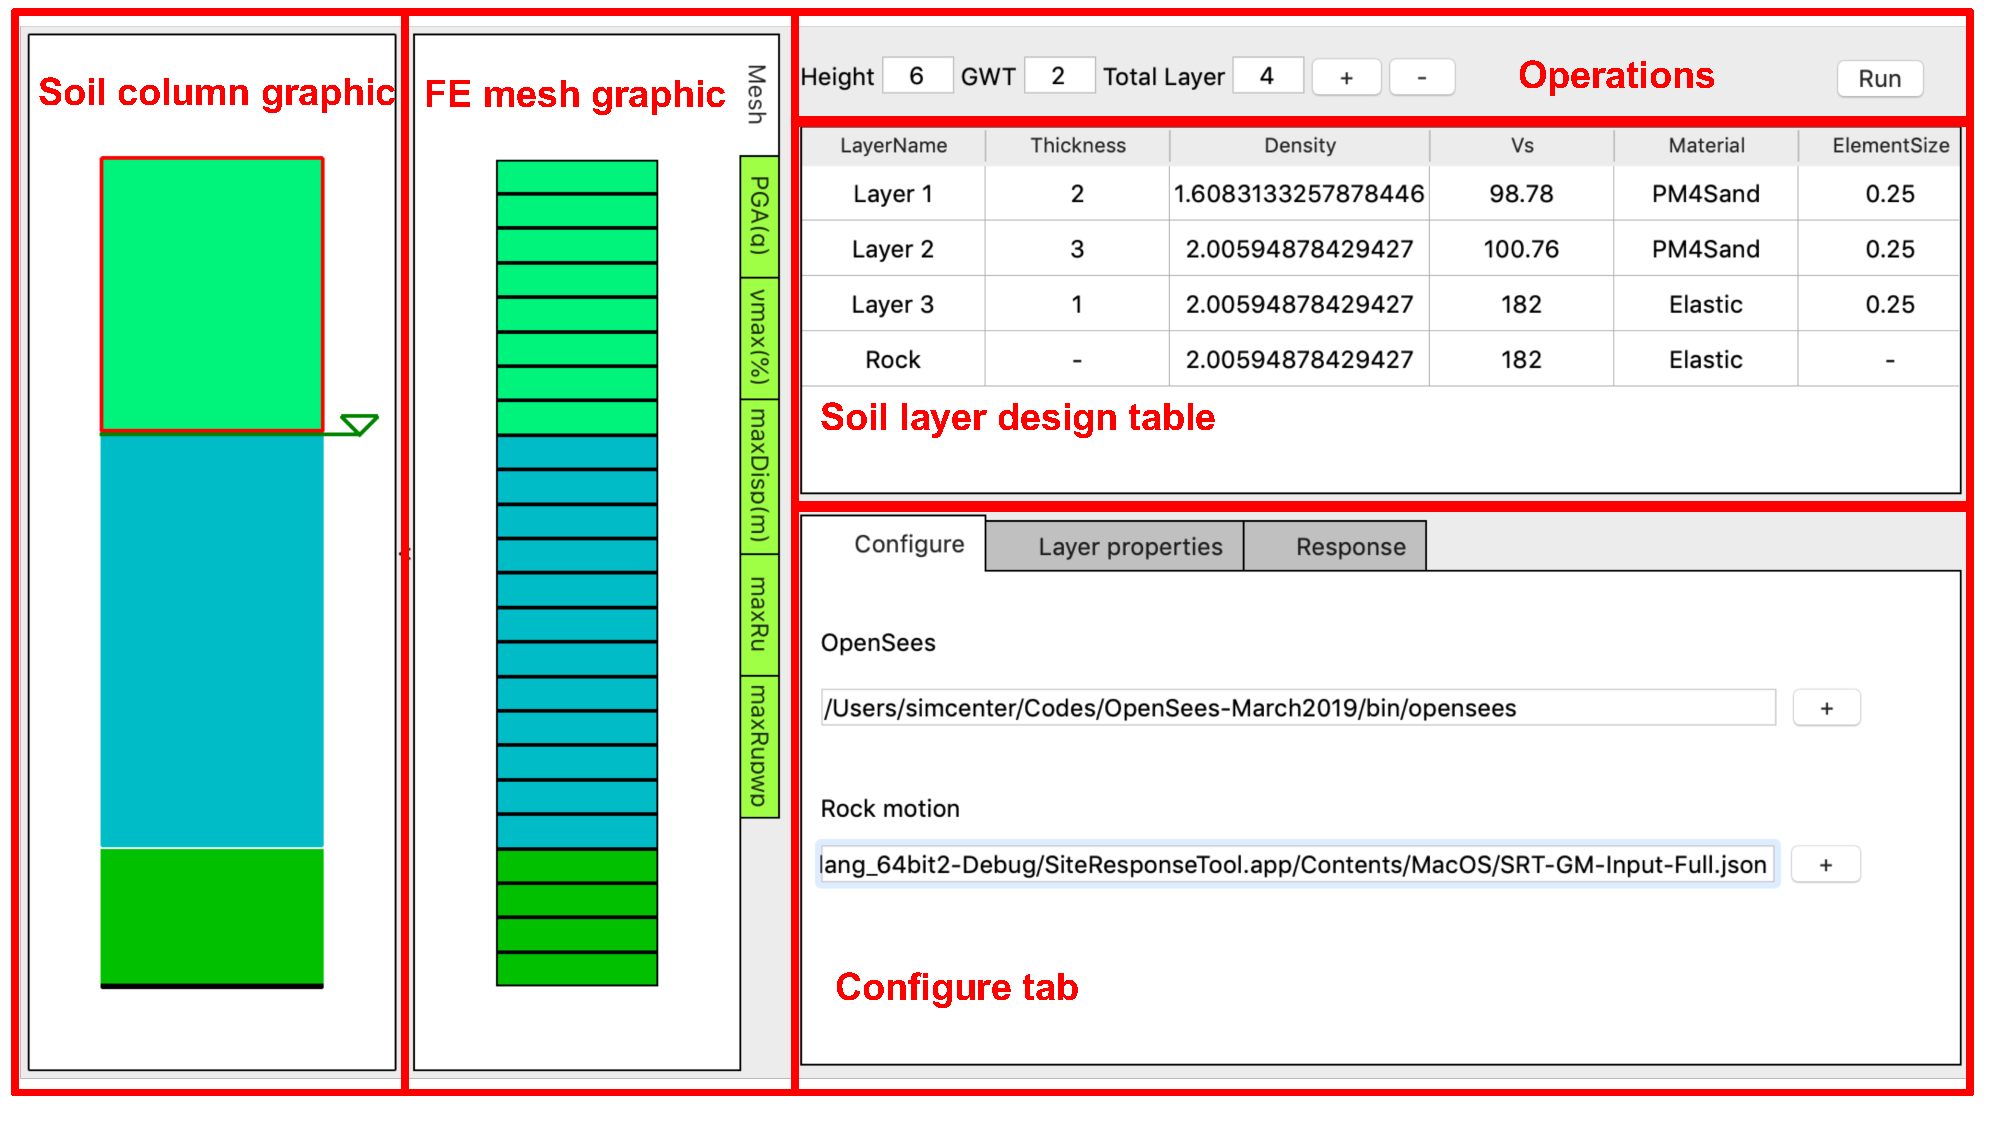
\includegraphics[width=0.8\textwidth]
    {usage/figures/s3hark1.pdf} }
  \caption{s$^3$hark - Panels}
  \label{fig:s3hark1}
\end{figure}

In the operation area as shown in \Cref{fig:s3hark2}, click the plus button to add a layer and the minors button to delete a selected layer. 
Change the ground water table in the GWT input field. 
In the configure tab, path of OpenSees executable and rock motion file need to be specified.
A click on the run button will start the finite element analysis.


\begin{figure}[!htbp]
  \centering {
    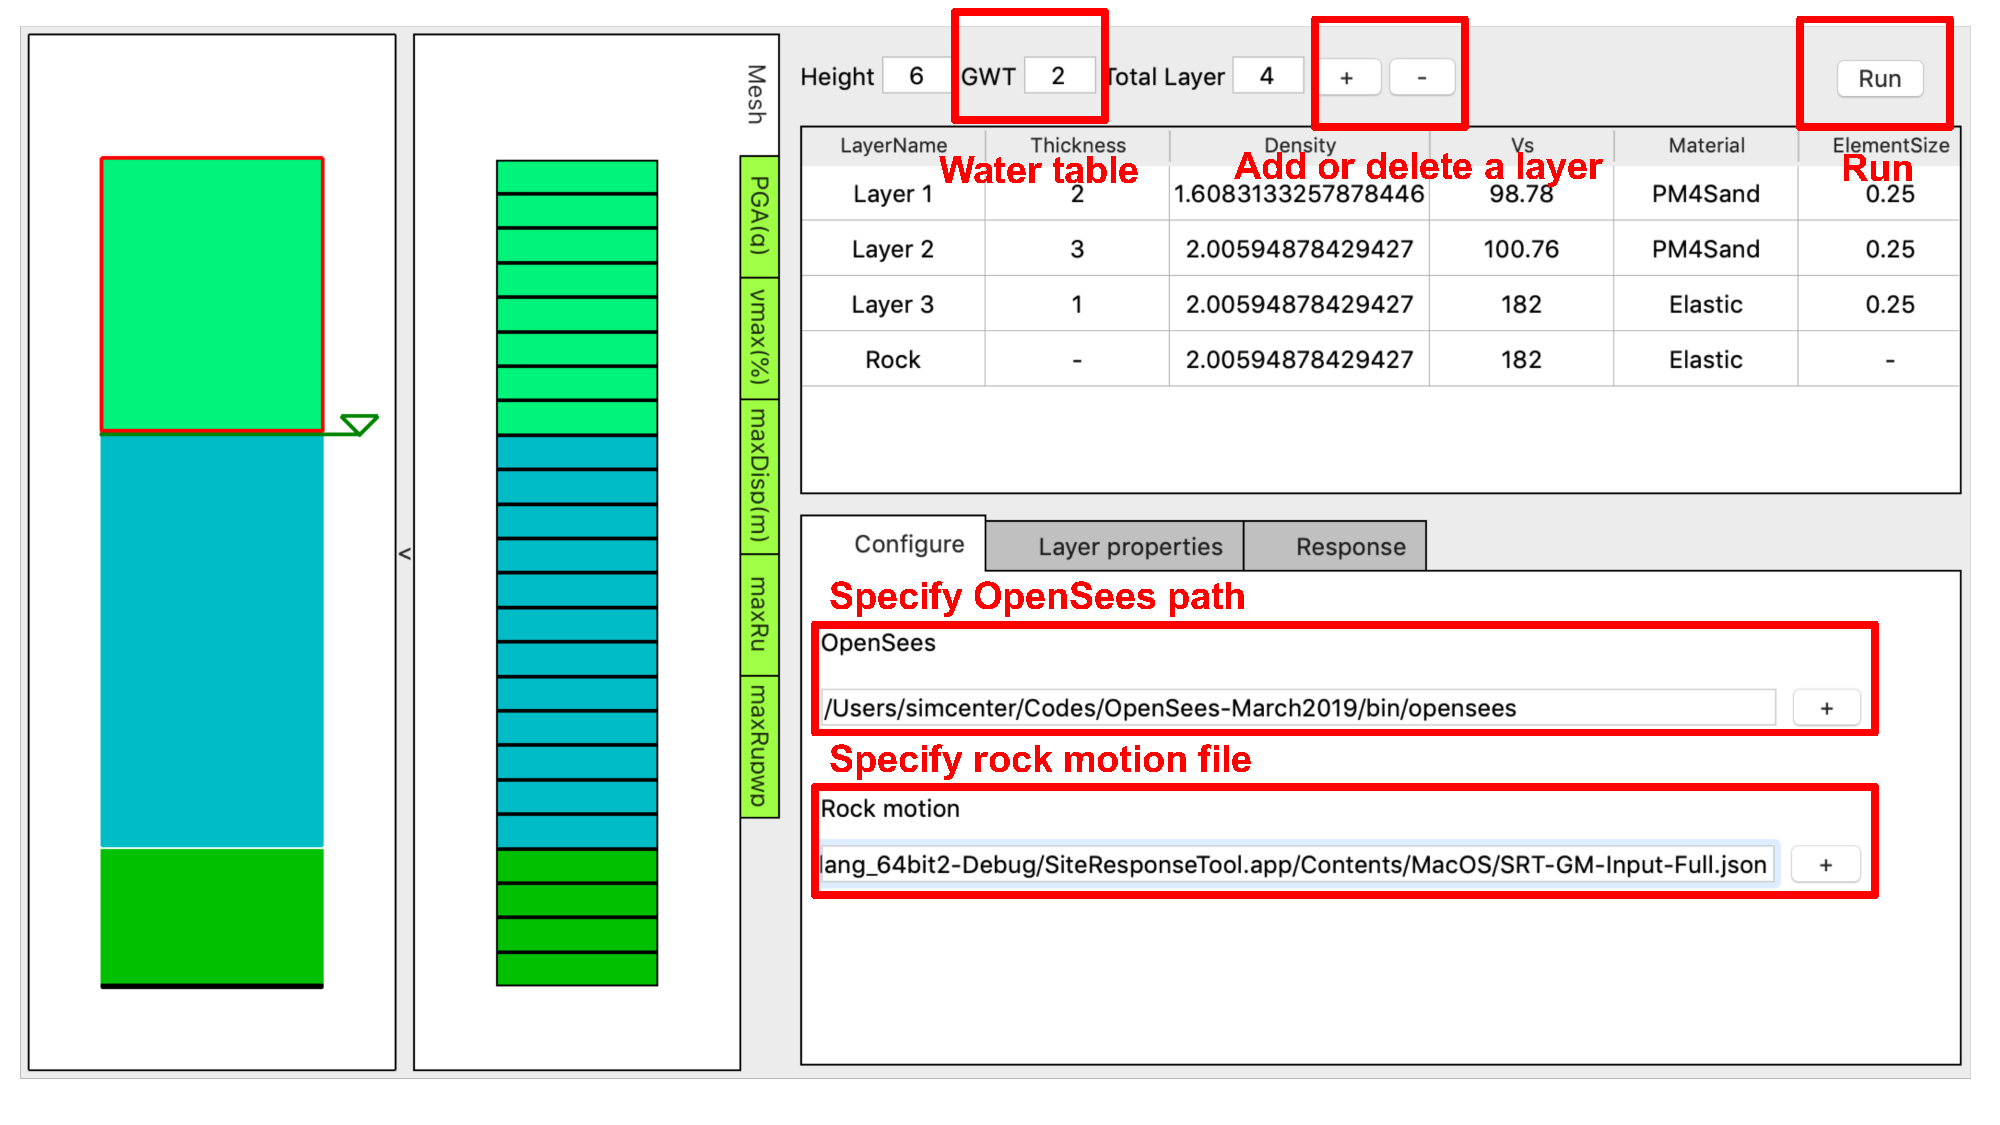
\includegraphics[width=0.8\textwidth]
    {usage/figures/s3hark2.pdf} }
  \caption{s$^3$hark - Configurations and Operations }
  \label{fig:s3hark2}
\end{figure}

Either click on the soil column or the table to select a layer \Cref{fig:s3hark3}. 
When a layer is selected, it will be highlighted in both the soil column graphic and the table. 
Selection of a soil layer will invoke the Layer properties tab, where the user can specify the material properties of this layer.
Double click on a cell of the table will allow the user to change the corresponding value.

\begin{figure}[!htbp]
  \centering {
    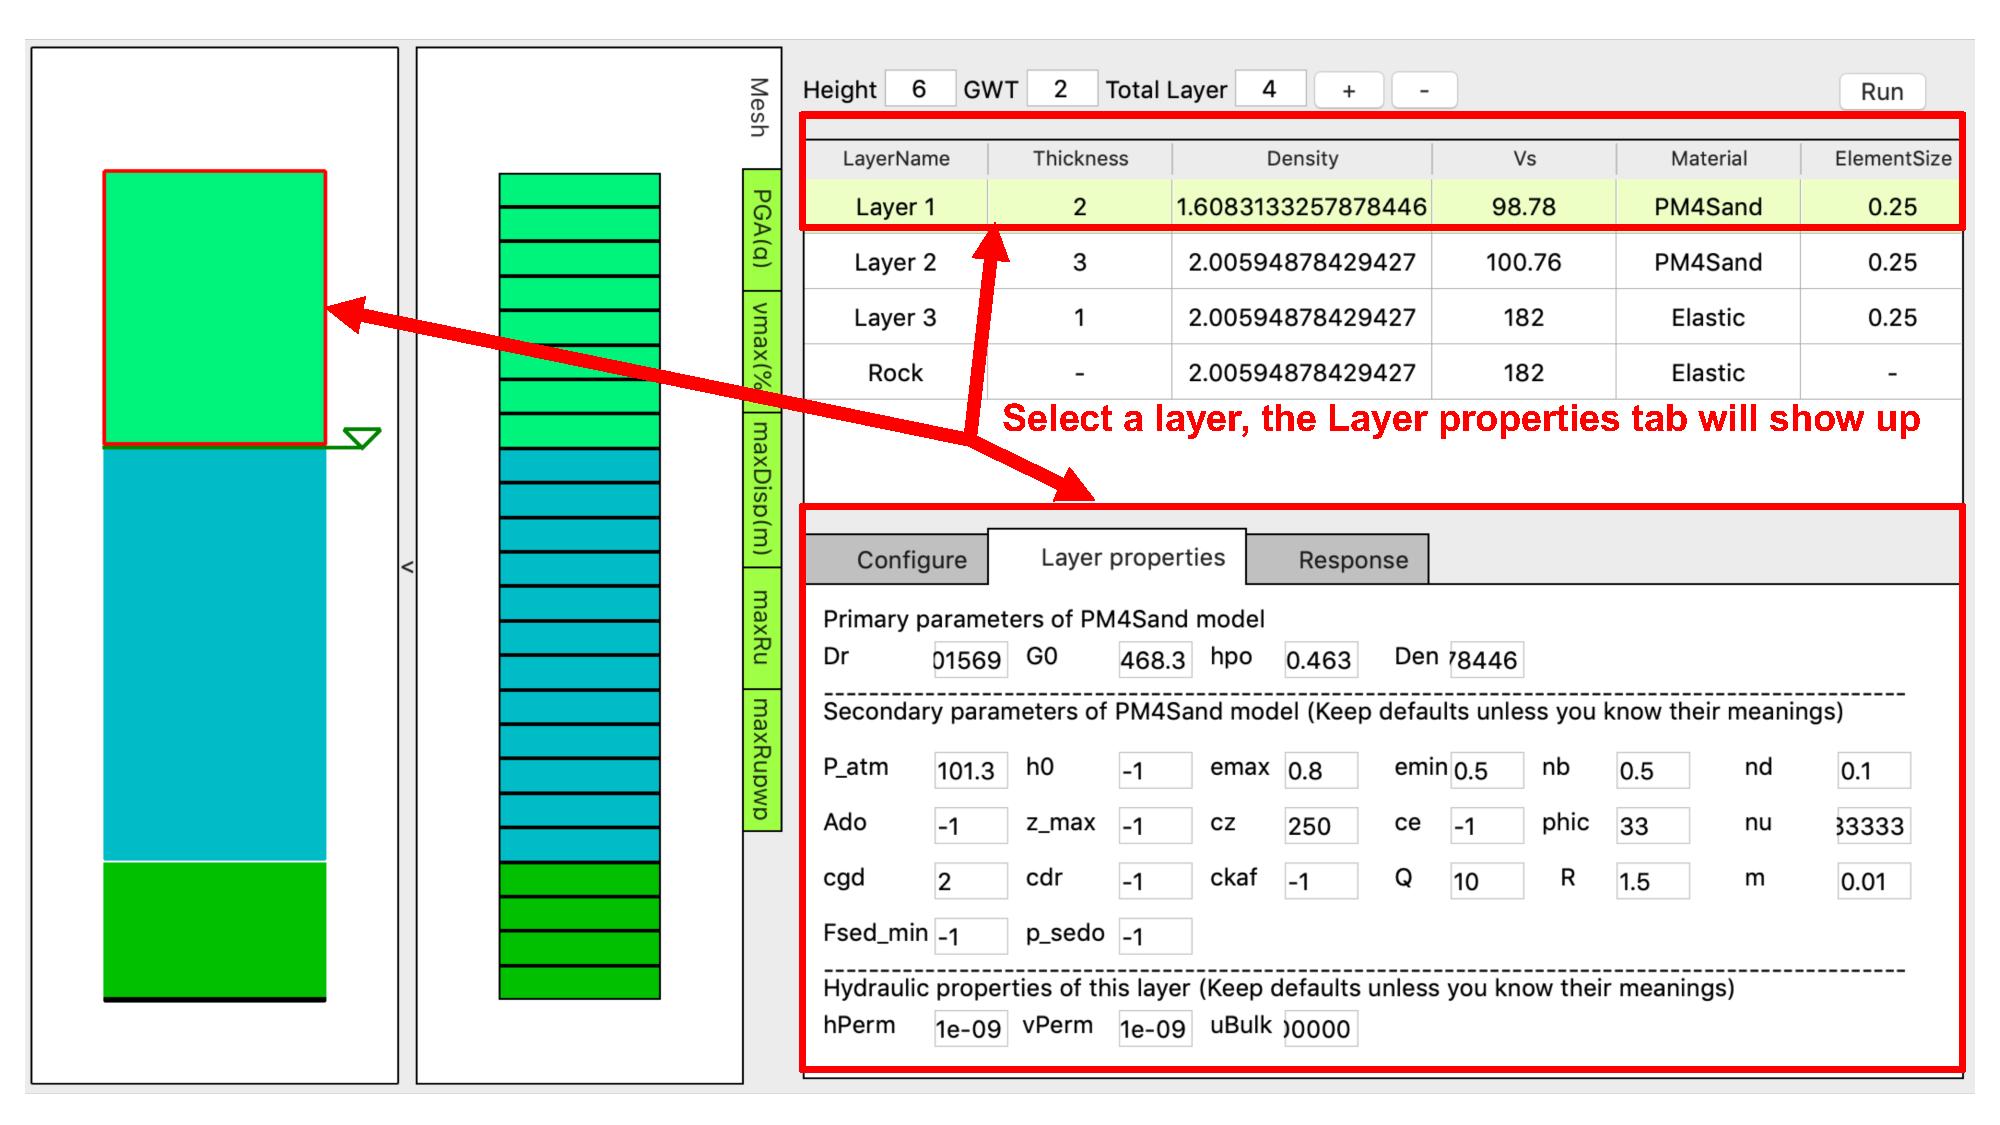
\includegraphics[width=0.8\textwidth]
    {usage/figures/s3hark3.pdf} }
  \caption{s$^3$hark - Layer modification }
  \label{fig:s3hark3}
\end{figure}


Upon the finish of the finite element analysis, the ground motion at the soil surface (\Cref{fig:s3hark4}) will be stored in EE-UQ's input file.
This computed motion will be later applied to the bottom of the building.

\begin{figure}[!htbp]
  \centering {
    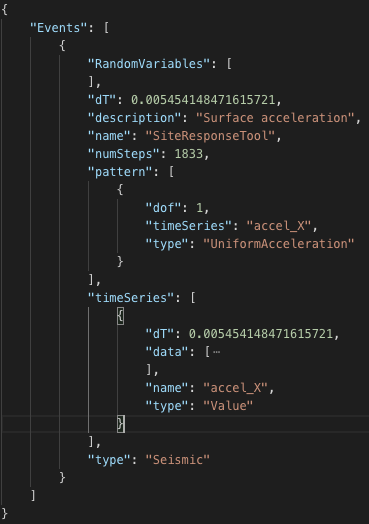
\includegraphics[width=0.4\textwidth]
    {usage/figures/s3hark4.png} }
  \caption{s$^3$hark - Surface motion }
  \label{fig:s3hark4}
\end{figure}


\subsection{User Application}
The final option for event definition is a user application. 
The user specifies the application name and the input file containing the specific input information 
needed by the application when it is running in the backend. 
As will be discussed later, when they use an additional application not provided, the user is also required 
to edit the tools registry file. There they must include a new event application with the same name 
and the location where that application can be found relative to the tools application directory. 
If running on DesignSafe, that application must be built and must be available on the Stampede2 supercomputer. 

Note: Given how DesignSafe runs the applications through Agave, the file permissions of this application must be 
world readable and executable (i.e., when a user runs their application through DesignSafe and Agave, they are not running it as themselves!)

\begin{figure}[!htbp]
  \centering {
    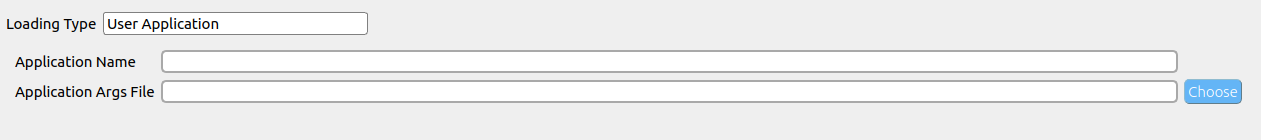
\includegraphics[width=1.0\textwidth]
    {usage/figures/userAppEvent.png} }
  \caption{User defined event}
  \label{fig:user_defined_event_panel}
\end{figure}



\section{FEM: Finite Element Method}
The FEM panel is intended to present users with a selection of FEM
applications that will take a building model generated by the BIM
application and the EVENT from the event application and perform a
deterministic simulation.  At present there is only one application
available, OpenSees and there is no application selection box.  That
will be modified in future versionsto allow user to provide their own
simulation application.  This is not the standard OpenSees executable,
but consists of a pre- and post-processor to take the BIM and EVENT
file and use OpenSees to determine the response, returning these
responses in an EDP.

For the OpenSees application the user is required to specify the
options to be used in the transient analysis. As shown \autoref{fig:fem},
this includes the choice of
\begin{enumerate}
\item Solution algorithm, the default is Newton Raphson.
\item Integration Scheme, the default is Newmarks linear acceleration
  method.
\item Convergence Test, the default is a norm on the unbalance force.
\item Convergence tolerance
\item Damping Ratio.
\end{enumerate}

\begin{figure}[!htbp]
  \centering {
    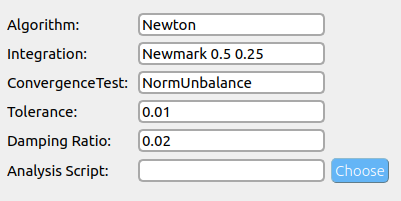
\includegraphics[width=0.8\textwidth]
    {usage/figures/fem.png} }
  \caption{Options for \texttt{OpenSees} transient analysis}
  \label{fig:fem}
\end{figure}

All the options available can be found in the OpenSees online user
manual.\\

A default transient analysis script is run with these inputs. It is
built for Version 3.0.0+ of OpenSees and uses a divide and conquer
algorithm in event of a convergence failure issue. This new algorithm
does not always work. \\

The user is also able to specify their own analysis script to run
instead of the default. When chosen the variables numStep and dt that
are obtained from the EVENT are set by the program. These variables
can be used by the user when providing their own analysis script.


\section{UQ: Uncertainty Quantification}
Throughout the input specification the user is defining variables. As
described in the above sections many of these variables can be
specified by the user to be random variables. The UQ panel is where the user specifies the distribution of these random variables. Besides the properties of random variables, the sampling method and the number of requested samples shall also be defined by the user. The panel is split, as shown
in \Cref{fig:uq_panel}, into two frames:

\begin{enumerate}
\item Sampling Methods 
\item Random Variables
\end{enumerate}

\begin{figure}[!htbp]
  \centering {
    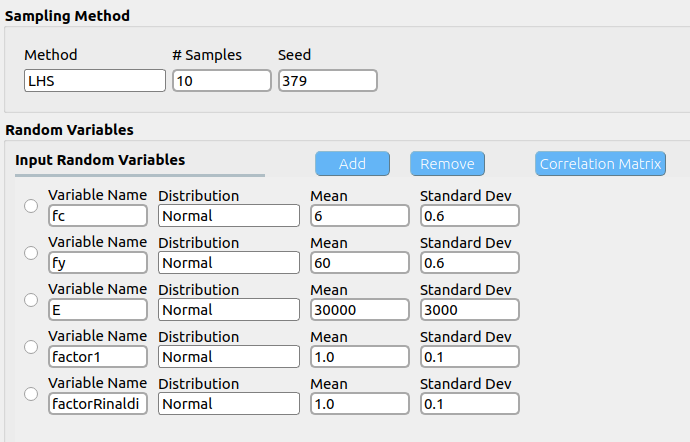
\includegraphics[width=0.8\textwidth]
    {usage/figures/uq1.png} }
  \caption{Uncertainty Quantification input panel}
  \label{fig:uq_panel}
\end{figure}

\subsection{Sampling Methods}
In the forward propagation problem, the user selects the sampling 
method to use from the dropdown menu \href{https://dakota.sandia.gov//sites/default/files/docs/6.9/html-ref/method-sampling.html}{sampling methods}. Currently there are five options available: 
Monte Carlo Sampling (MCS),  Latin Hypercube Sampling (LHS), Importance Sampling (IS), and sampling based on surrogate models, including Gaussian Process Regression (GPR) and Polynomial Chaos Expansion (PCE). Depending on the option selected, the user must specifies the appropriate input parameters for each. For instance, for MCS, the number of samples specifies the number of simulations to be performed, and providing a random seed allows the user to reproduce the same set of samples from the random variables multiple times.

\begin{figure}[!htbp]
  \centering {
    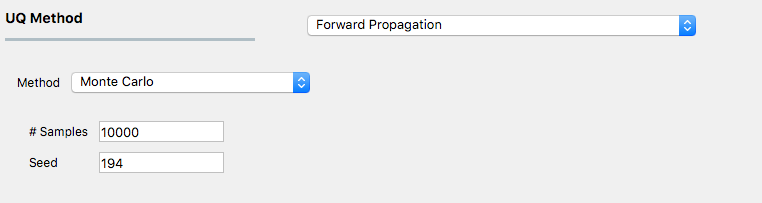
\includegraphics[width=1.0\textwidth]
    {examples/fig_quofem/fw_mc.png} }
  \caption{Monte Carlo Sampling input panel}
  \label{fig:mcs}
\end{figure}

Figure \Cref{fig:mcs} shows the input panel corresponding to the Monte Carlo Sampling (MCS) setting. Two input parameters need to be specified, the number of samples to be executed, as well as the seed used in generating the random samples. 


\begin{figure}[!htbp]
  \centering {
    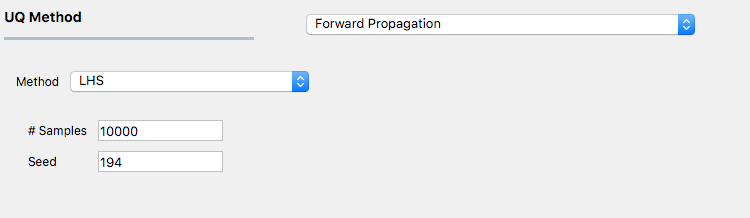
\includegraphics[width=1.0\textwidth]
    {examples/fig_quofem/fw_lhs.png} }
  \caption{Latin Hypercube Sampling input panel}
  \label{fig:lhs}
\end{figure}

Figure \Cref{fig:lhs} shows the input panel corresponding to the Latin Hypercube Sampling (LHS) scheme. Two input parameters also need to be specified, the number of samples to be executed, as well as the seed used in generating the LHS samples. 

\begin{figure}[!htbp]
  \centering {
    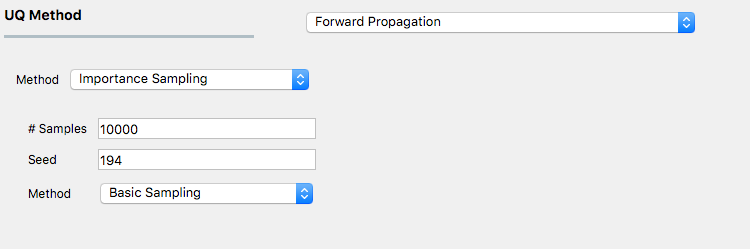
\includegraphics[width=1.0\textwidth]
    {examples/fig_quofem/fw_is.png} }
  \caption{Importance Sampling input panel}
  \label{fig:is}
\end{figure}

For rare event analysis, Figure \Cref{fig:is} shows the input panel for Importance Sampling (IS) scheme. Similar to MCS and LHS, the IS requires both the number of samples to be executed and the corresponding seed for generating such random samples. In addition, the Importance Sampling algorithm can performed via three different approaches, as specified by the third input method. The latter includes Basic Sampling, Adaptive Sampling, and Multimodal Adaptive Sampling. 


For uncertainty propagation with surrogates, two popular surrogates are available, namely Gaussian Process Regression (GPR) and Polynomial Chaos Expansion (PCE). Figure \Cref{fig:gpr} shows the input panel for the GPR model, with input panels for training and sampling. 

\begin{figure}[!htbp]
  \centering {
    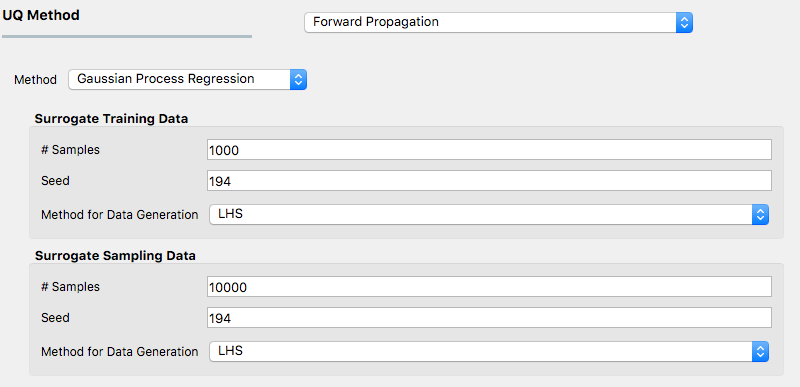
\includegraphics[width=1.0\textwidth]
    {examples/fig_quofem/fw_gp.png} }
  \caption{GPR forward propagation input panel}
  \label{fig:gpr}
\end{figure}

For uncertainty propagation with Gaussian Process Regression (GPR), Figure \Cref{fig:gpr} shows the input panel for the PCE model, with input panels for training and sampling as well. The first set of input parameters in the surrogate training data specify the dataset used for training the surrogate model, while the second set of input parameters in the surrogate sampling data relate to the dataset used for sampling the surrogate. Care must be taken in specifying the training dataset to results in an accurate response surface approximation. 

\begin{figure}[!htbp]
  \centering {
    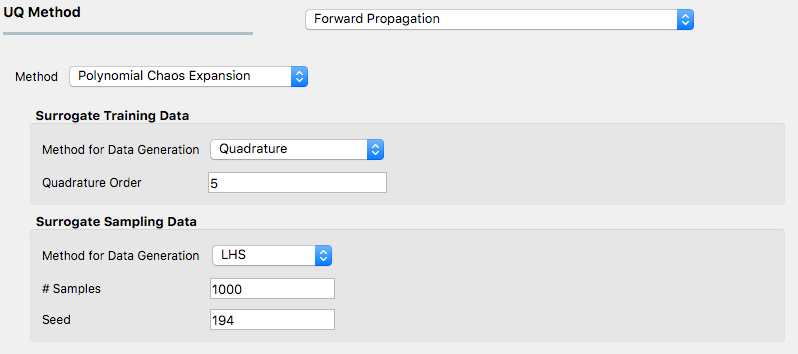
\includegraphics[width=1.0\textwidth]
    {examples/fig_quofem/fw_pce.png} }
  \caption{PCE forward propagation input panel}
  \label{fig:pce}
\end{figure}

For uncertainty propagation with Polynomial Chaos Expansion (PCE), Figure \Cref{fig:pce} shows the input panel for the PCE model, with input panels for training and sampling as well, similar to the input GPR panel. The first set of input parameters in the surrogate training data specify the dataset used for training the surrogate model, while the second set of input parameters in the surrogate sampling data relate to the dataset used for sampling the surrogate. Extreme care must be taken in specifying the parameters of the training dataset to results in an accurate response surface approximation. 

If you are not sure about the training parameters of the surrogates, please refrain from using the surrogates for forward propagation and use instead conventional sampling such as MCS and LHS as discussed above. 

\subsection{Reliability Analysis}

For reliability analysis, figure \Cref{fig:rel} shows the input panel for the reliability capabilities. Currently, both First-Order Reliability Methods (FORM) and Second-Order Reliability Methods (SORM) are supported. The user can specify the local or global solution in the Reliability Scheme input parameter. In addition, the user needs to specify the method for searching for the Most Probable Point (MPP); if not sure, do not use any MPP approximation. 

For both first and second-order reliability analysis, the user needs to specify the either the response levels or the probability levels at which the CDF of the QoI needs to be queried. The user can specify multiple query points, separated by a space. 


\begin{figure}[!htbp]
  \centering {
    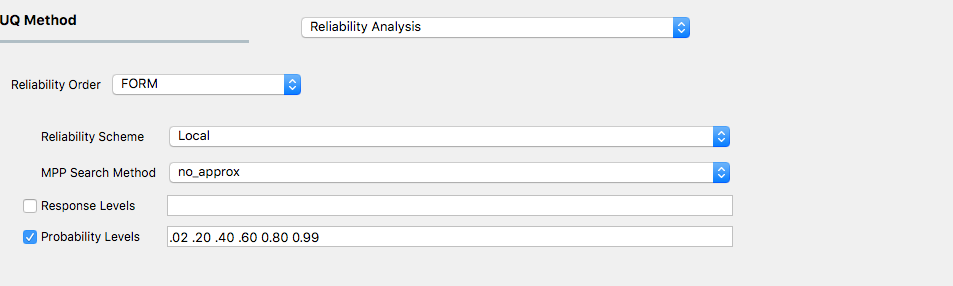
\includegraphics[width=1.0\textwidth]
    {examples/fig_quofem/rel_form.png} }
  \caption{Reliability input panel}
  \label{fig:rel}
\end{figure}




\subsection{Random Variables}
The RV panel allows the user to specify the probabilistic distribution for the random problem at hand. The following probabilistic distributions for the random variables are currently supported: 
\begin{enumerate}
\item Gaussian
\item Lognormal
\item Beta
\item Uniform
\item Weibull
\item Gumbell
\end{enumerate}

Each distribution has different parameters, and the user needs to select accordingly the parameters for the distribution selected for each random variable. Once the user selects the distribution of the random variable, the
corresponding input boxes for the parameters will show. 

\Cref{fig:rv} shows the panel for a problem with four Random Variables with all random input following Gaussian distributions. 

\begin{figure}[!htbp]
  \centering {
    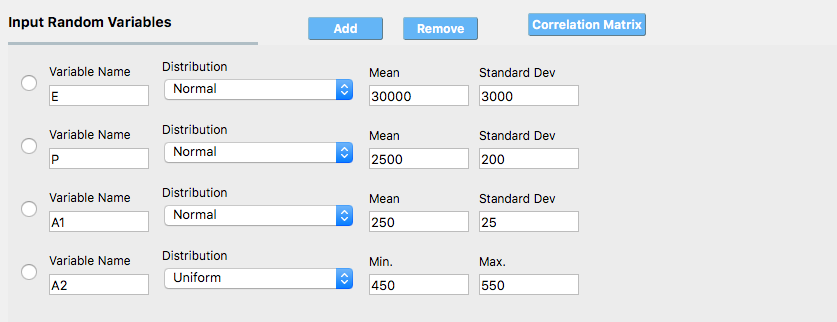
\includegraphics[width=0.8\textwidth]
    {examples/fig_quofem/rv.png} }
  \caption{Random Variable specification}
  \label{fig:rv}
\end{figure}





\section{EDP: Engineering Demand Parameters}
This panel is where the user selects which outputs will be displayed when
the simulation runs. There are two options available in the pull-down
menu:
\begin{enumerate}
  \softwareSwitch{WE-UQ}{
    \item Standard Wind (\Cref{subsec:sectionStandardWind})    
  }{
    \item Standard Earthquake (\Cref{subsec:sectionStandardEarthquake})    
  }
\item User Defined (\Cref{subsec:sectionUserDefined})
\end{enumerate}

\softwareSwitch{WE-UQ}{
  \subsection{Standard Wind}\label{subsec:sectionStandardWind}
  When the user selects Standard Wind there are no additional
  inputs required. The standard wind EDP generator will ensure the
  the max absolute value of the following are obtained:  
}{
  \subsection{Standard Earthquake}\label{subsec:sectionStandardEarthquake}
  When the user selects Standard Earthquake there are no additional
  inputs required. The standard earthquake EDP generator will ensure the
  the max absolute value of the following are obtained:  
}
\begin{enumerate}
\item Relative Floor displacements:
\item Absolute Floor Accelerations
\item Interstory Drifts
\end{enumerate}

The results will contain results for these in abbreviated form:
\begin{itemize}
\item PFD peak relative floor displacement $1-PFD-FLOOR_CLINE$
\item PFA peak floor acceleration (relative + ground motion):
  $1-PFA-FLOOR-CLINE$
\item PID peak inter-story drift: $1-PID-STORY-CLINE$
\end{itemize}

NOTE: Floors are numbered starting at floor 0, and stories are numbered starting at story 1.

\subsection{User Defined}\label{subsec:sectionUserDefined}
As shown in \Cref{fig:userEDP}, this panel allows the user to determine their own output and process it. When using this option the user provides additional data:

\begin{figure}[!htbp]
  \centering {
    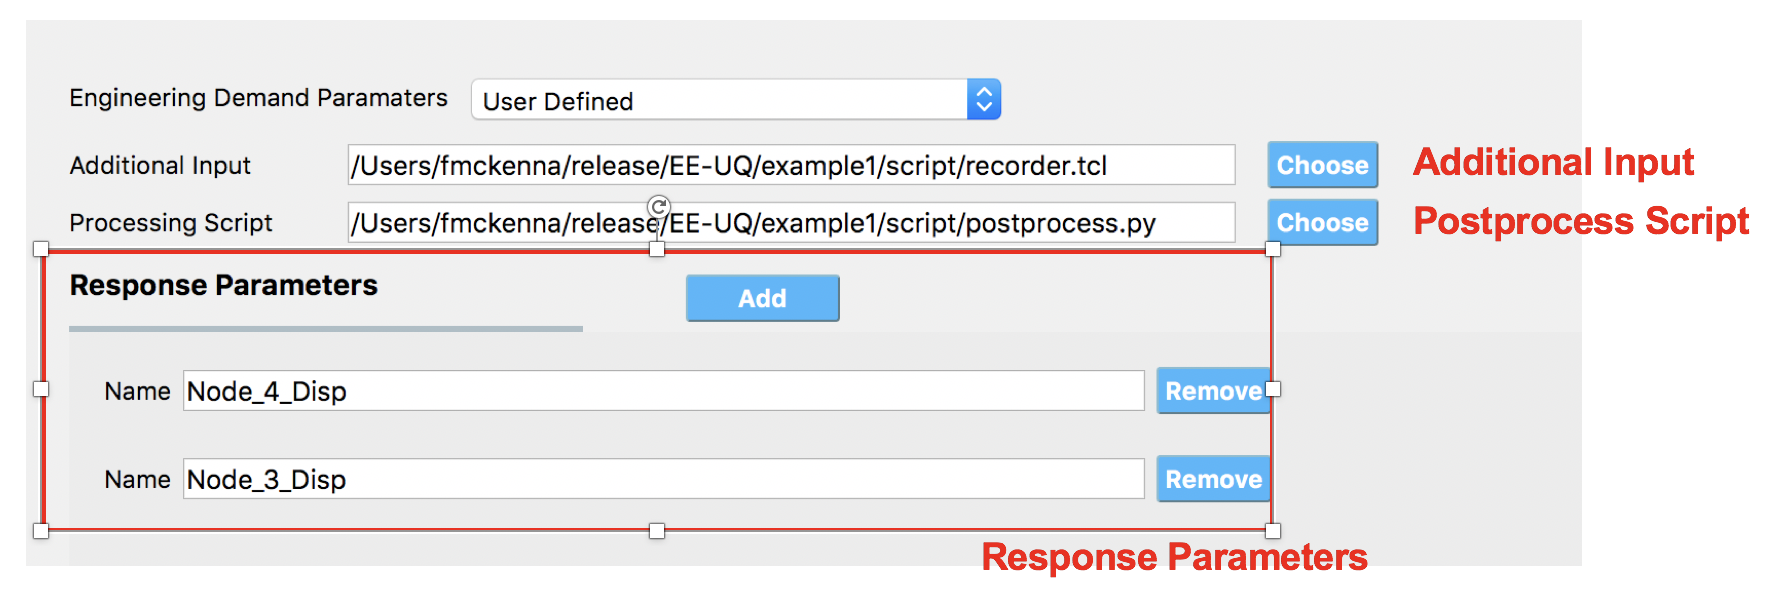
\includegraphics[width=0.8\textwidth]
    {usage/figures/userDefinedEDP.png} }
  \caption{userEDP}
  \label{fig:userEDP}
\end{figure}

\begin{enumerate}
\item Additional Input: These are additional commands that are invoked
  by the analysis application before the transient analysis is
  performed. For example, for OpenSees this would be a script
  containing a series of recorder commands. \\

A recorder file passed to OpenSees might look like the following:
\begin{verbatim}
recorder EnvelopeNode -file node.out -node 1 2 3 4 -dof 1 disp
recorder EnvelopeElement -file ele.out -ele 1 2 3 forces
\end{verbatim}

\item Postprocess Script: This is a python script that will be invoked
  after the finite element application has run. It must be provided by
  the user. It's purpose is to process the output files and create a
  single file, results.out. This file must contain a single line with
  as many entries as EDP's specified.

For example, a postprocessing file that would take the outputs from the analysis to create the results file might look like the following:

\begin{python}
#!/usr/bin/python                                                                 

import sys
import re

EDPs = ['Node_4_Disp', 'Node_3_Disp']

inputArgs = sys.argv

with open ('node.out', 'rt') as inFile:
    line = inFile.readline()
    line = inFile.readline()
    line = inFile.readline()
    displ = line.split()
    numNode = len(displ)

inFile.close

#                                                                                 
# now process the input args and write the results file                           
#                                                                                 

outFile = open('results.out','w')

#                                                                                 
# note for now assuming no ERROR in user data                                     
#                                                                                 

for i in EDPs[0:]:
    print i
    theList=i.split('_')

    if (theList[0] == 'Node'):
        nodeTag = int(theList[1])

        if (nodeTag > 0 and nodeTag <= numNode):
            if (theList[2] == 'Disp'):
                nodeDisp = displ[nodeTag-1]
                outFile.write(nodeDisp)
                outFile.write(' ')
            else:
                outFile.write('0. ')
        else:
            outFile.write('0. ')
    else:
        outFile.write('0. ')

outFile.close
\end{python}



\item Response Parameters. This is an area in which the user
  associates a variable name with the column of the results output
  file. If the process script has an array of strings named named
  EDP's the script, the Response Parameters will be initially set with
  these values from the script.
\end{enumerate}



\section{RES}
When the user hits the Run button, and assuming the results are
successful. The results are presented here.  A successful run or
download of a job that ran successfully will result in 3 tabbed
widgets being displayed in this panel.  The first panel shows summary
statistics: mean and stdDev values or min-max values if discrete set,
i.e. multiple events for each of the EDP's specified in the EDP panel.

\begin{figure}[!htbp]
  \centering {
    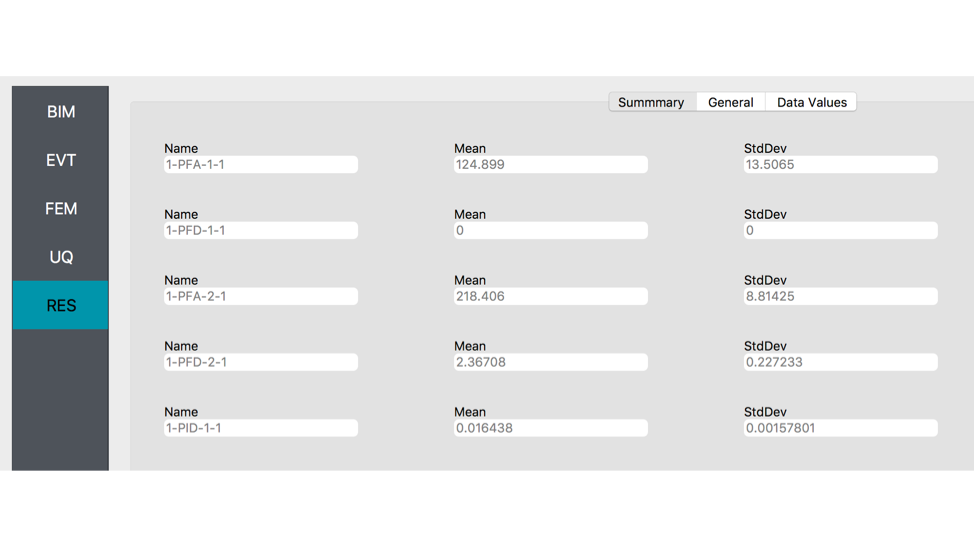
\includegraphics[width=0.8\textwidth]
    {figs/Figure12.png} }
  \caption{RES}
  \label{fig:figure12}
\end{figure}

The second panel shows the summary information.

\begin{figure}[!htbp]
  \centering {
    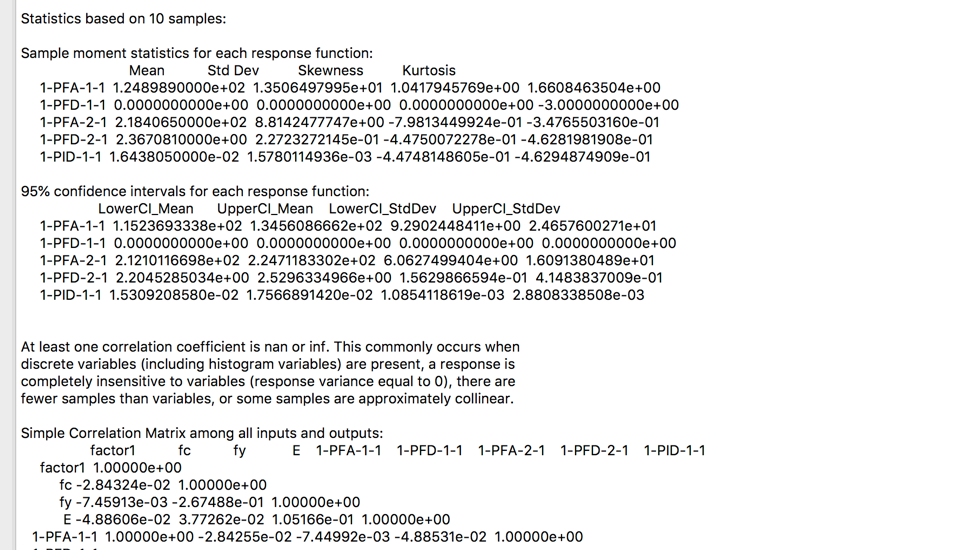
\includegraphics[width=0.8\textwidth]
    {figs/Figure13.png} }
  \caption{RES General tab}
  \label{fig:figure13}
\end{figure}

The third panel presents graphically and in tabular form the
results. By selecting different columns with left and right mouse
buttons in the table below the graphic, the information in the graph
is changed. Selecting the left mouse button changes the Y axis, the
right mouse changes the X axis. If the same column is selected using
both left and right keys, the CDF and PDF is displayed. If last mouse
press was with the left button, the PDF and if right the CDF.
 
As for the columns. You will see a column for each random variable the
workflow came across. There may be more than you specified if the
applications want the UQ engine to consider their own variables in the
computation. The outputs at present are limited to:

\begin{figure}[!htbp]
  \centering {
    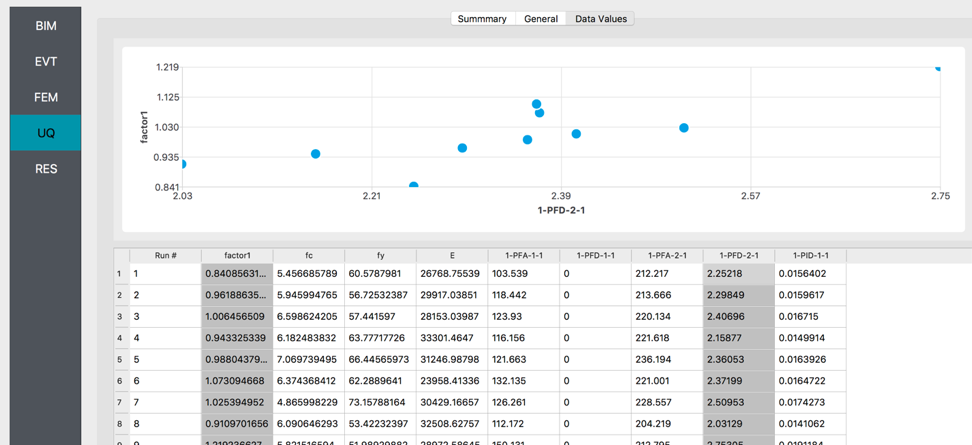
\includegraphics[width=0.8\textwidth]
    {figs/Figure14.png} }
  \caption{UQ Data Values}
  \label{fig:figure14}
\end{figure}


\section{Push Buttons}
There are a number of buttons in the Push Button area of \autoref{fig:figure1}:
\subsection{RUN – to run the simulation of the user’s desktop machine.}
\begin{figure}[!htbp]
  \centering {
    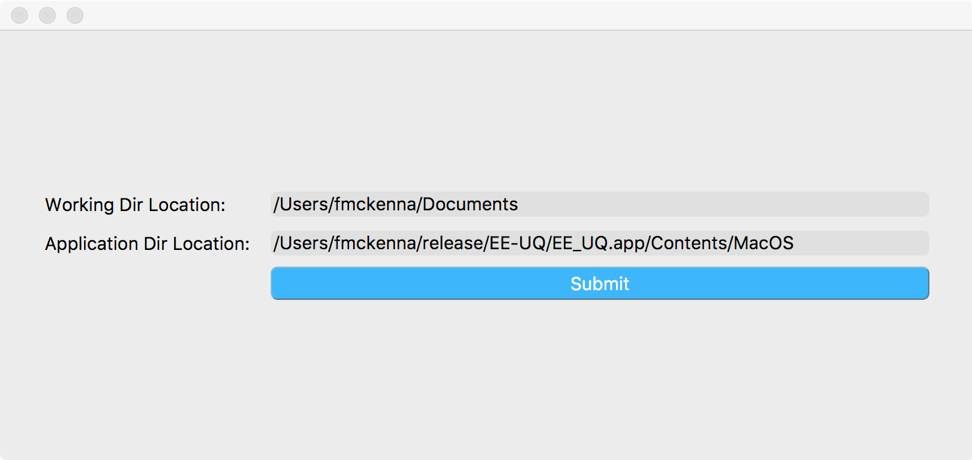
\includegraphics[width=0.8\textwidth]
    {figs/Figure15.png} }
  \caption{Run button}
  \label{fig:figure15}
\end{figure}
The window that pops up is as shown in \autoref{fig:figure15}. There are 2 entries and a push button: 

\begin{itemize}
\item Working Dir Location: specifies where the $EE_UQ$ application can create a “temporary” directory called tmp. SimCenter that the application 
creates when the submit button is pressed. The application creates this directory, copies files to it that the application needs as a result of your 
input (e.g. if you are using OpenSees input script, it will to the tmp. SimCenter directory copy that script, ALL FILES IN THAT DIRECTORY AND ALL FILES IN 
SUBDIRECTORIES OF THAT DIRECTORY GET COPIED SO DON’T PLACE THE SCRIPT IN HOME, DOWNLOADS, DOCUMENTS, ….
\item Application Dir Location: SHOULD NOT BE TOUCHED unless you are introducing your own applications or want to build and modify the 
applications provided with the tool. It is this directory the application tool looks to find the applications to run.
\end{itemize}


Finally, when inputs are finished the user hits submit button to start the backend job. If it runs the window will close and the RES 
panel will pop up on successful run. Do not press the submit button multiple times while waiting for it to close. We cannot guarantee 
what will happen and we did not disable the button in this release.

\subsection{RUN at DesignSafe}
Click this button to process the information, and send to DesignSafe where the job will be run on a supercomputer and results stored in your DesignSafe jobs folder.

\begin{figure}[!htbp]
  \centering {
    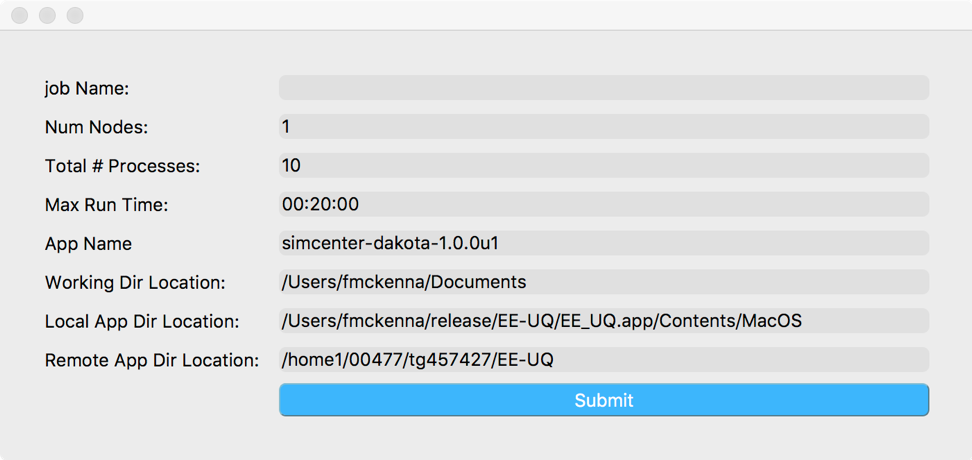
\includegraphics[width=0.8\textwidth]
    {figs/Figure16.png} }
  \caption{Remote button}
  \label{fig:figure16}
\end{figure}

A similar bit longer input panel is brought up:
\begin{itemize}
\item JobName: The name the user can use to identify the job in Get from DesignSafe.
\item NumNodes: The number of compute nodes to use on Stampede2. Using the default App Name the job will run on Stampede2’s KNL Landing (KNL) 
compute nodes. Each node has 68 cores. The actual number of cores the application will use on each of these nodes depends on the total number of 
processes specified. As per the TACC webpage, for MPI tasks it’s best not to specify more than 64-68 processes to run. Depending on the numerical 
computations and amount of memory each uses, so as to avoid page faulting, for large simulations you may wish to use more nodes and less processes.
\item Total Number of Processes: Total number of MPI parallel processes the UQ engine is going to use.
\item Max Wall Time:  HOURS:MIN:SEC be conservative. Your job is killed after the time limit. On Stampede2 you have a max wall time of 24 hours.
\item App Name:   Name of Agave app to run. DO not touch unless you know what you are doing.
\item Working Dir Location: specifies where the $EE_UQ$ application can create a “temporary” directory called tmp. SimCenter that the application 
creates when the submit button is pressed. The application creates this directory, copies files to it that the application needs as a result of your 
input (e.g. if you are using OpenSees input script, it will to the tmp. SimCenter directory copy that script, ALL FILES IN THAT DIRECTORY AND ALL FILES 
IN SUBDIRECTORIES OF THAT DIRECTORY. (SO, DON’T PLACE THE SCRIPT IN HOME, DOWNLOADS, DOCUMENTS, …). That directory is removed when jib has been successfully submitted.
\item Local App Dir Location: SHOULD NOT BE TOUCHED unless you are introducing your own applications or want to build and modify the applications 
provided with the tool. It is this directory the application tool looks to find the applications it needs.
\item Remote App Dir Location: Remote directory on Stampede2 where applications needed by workflow reside. DO not touch unless you know what you are doing.

\end{itemize}


\subsection{GET from DesignSafe}
	Click this button to obtain from DesignSafe your list of jobs and select from that list a job to update status of, download or delete.

\subsection{Exit}
Click this button to exit the application. 
